\section{Deanonymization Attacks and Their Implications}
In this section we survey deanonymization attacks on Bitcoin, which can roughly be characterized into the following four categories based on the source of information:
\begin{enumerate}
	\item Collapsing multi-input transactions to the same owning entity or user,
	\item Bitcoin value flow through the transaction graph (defined below),
	\item Side-channel attacks that rely on timing and network-layer (e.g., IP addresses) information, and
	\item Auxiliary information linkability (e.g., entity-to-address linking using information acquired via external mediums).
\end{enumerate}
Our analysis is based on the small body of work primarily analyzing the first three classes of attacks. The last class is generally not discussed in scholarly work, but rather in popular media. Before discussing such attacks, we first describe the attack vectors leveraged by researchers and malicious users while forming such attacks.

\subsection{Attack Vectors} \label{sec:vectors}
Given the design of the Bitcoin system, it may seem surprising that the surface for privacy- and anonymity-targeting attacks is quite large. In fact, there is a large amount of information available to attackers that may be, and has been, exploited to carry out such attacks. Perhaps most fruitful are the \emph{transaction} and \emph{user} graphs that can be constructed via network and transaction analysis. The transaction graph is a directed graph $\mathcal{T}$ with a vertex set $V(\mathcal{T})$ containing all transactions in the Bitcoin history and edge set $E(\mathcal{T})$ containing directed edges between the source (sender) and target (recipient) for each transaction. The user graph is yet another directed graph $\mathcal{U}$ with a vertex set $V(\mathcal{U})$ corresponding to physical users, or entities, partaking in the Bitcoin system and edge set $E(\mathcal{U})$ corresponding to the flow of Bitcoins or funds between two users. With sufficient network analysis (i.e., eavesdropping on Bitcoin traffic in the network), one may also construct a \emph{network address} graph, which is similar to the user graph with the exception that vertices represent physical IPs instead of particular users. 

% \begin{figure}
% \begin{center}
% 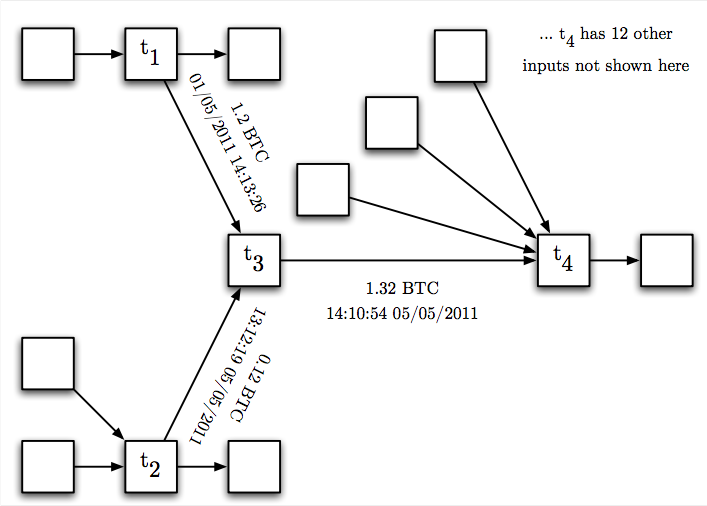
\includegraphics[scale=0.35]{images/transaction_graph.png}
% \caption{A sample transaction graph \protect\cite{ReidHarrigan13}.}
% \label{fig:transaction-graph}
% \end{center}
% \end{figure}

% \begin{figure}
% \begin{center}
% 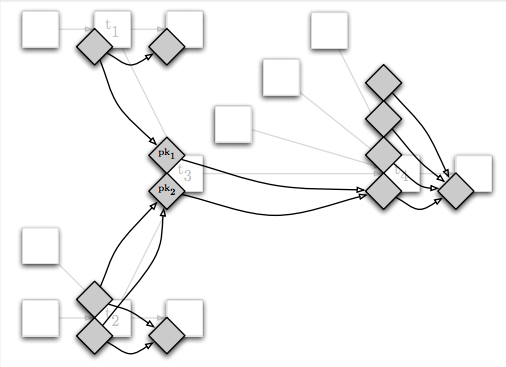
\includegraphics[scale=0.45]{images/transaction_user_graph.png}
% \caption{A sample user graph \protect\cite{ReidHarrigan13}.}
% \label{fig:user-graph}
% \end{center}
% \end{figure}

\subsection{Detailed Anonymization Attacks and Analysis Techniques} \label{sec:attacks}
%Current loss of privacy through voluntary identification/off network information, flow analysis, IP tracking. Needs more info

Intuitively, a successful attack on the anonymity of Bitcoin yields a mapping between Bitcoin addresses, or public keys, to their respective owners. Depending on the success criteria for such an attack, the attacker may seek to find a single mapping for a particular user or, quite oppositely, a mapping for as many users as possible. Accordingly, there has been substantial research investigating the degree to which anonymity is achieved \cite{ReidHarrigan13,BetterToBitter,Fistful12,Shamir13-bitcoingraph,Androulaki12-privacy}; proposed solutions presented in the literature are discussed in the following section.

Although the original Bitcoin proposal suggests that anonymity, or rather pseudonominity, is possible due to the expected difficulty of associating Bitcoin addresses with their physical owners, there have been ample works attempting to disprove this claim. In fact, one of the earliest anonymity analyses was done by Dan Kaminsky in 2011, a well-known security consultant and researcher. He assessed the anonymity claims of Bitcoin by performing the following experiment: He began by opening up a connection to a large set of peers in the Bitcoin network. Under the assumption that the first appearance of a transaction stems from the original sender (unless an anonymizing layer such as Tor is used to obscure the source), it became fairly easy to combine the peer connections with some elementary traffic analysis to derive a mapping between Bitcoin addresses and IP-layer addresses \cite{kaminsky}. While IPs are rarely static due to DHCP and mobile devices, it is not a significant leap to suspect that such knowledge could reveal the underlying user's identity, especially if offline information is used (e.g., if the attacker is able to correlate the IP addresses to users using public forums or other applications). With this observation, a more active deanonymization attack, as carried out by Kaminsky \cite{kaminsky,ReidHarrigan13}, would involve malicious nodes scanning for Bitcoin clients listening to port TCP/8333 and open a direct connection. While proxy services like Tor can hide outbound connections, an inbound connection will not be obfuscated. By listening to transaction announcements over time, the client that first reports a transaction is the one that initiated it. This allows the malicious nodes to link transactions to IP addresses.

While using Tor enables one to obfuscate the source of a transaction, it does not solve the problem entirely for several reasons. First, Tor does not provide perfect source secrecy. Tor is inherently susceptible to \emph{end-to-end correlation attacks} in which the attacker controls both ends of a Tor circuit used to send data. Second, Tor was designed for low-latency, high throughput anonymous traffic. As such, it is susceptible to side channel timing attacks \cite{bitcoin-tor-wiki}.

\begin{figure}
\begin{center}
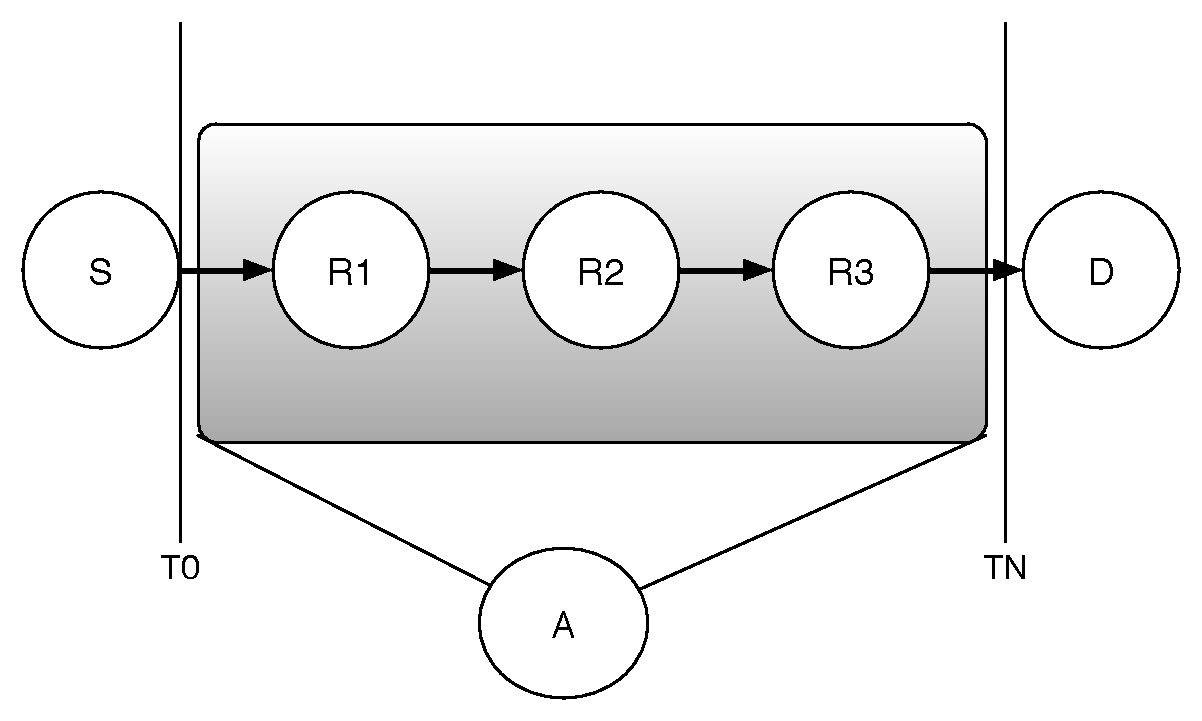
\includegraphics[scale=0.40]{images/tor_attack.pdf}
\label{TODO.}
\label{fig:tor-end-to-end}
\end{center}
\end{figure}

Trivial attacks on privacy and anonymity involve using the Bitcoin block chain to follow all the transactions associated with that address. As user commonly have many addresses, a more sophisticated attack requires the adversary to link the known address with other hidden addresses and then analyze the transactions associated with those addresses. The two major heuristics for linking addresses are \emph{multi-address transactions} and \emph{shadow or change addresses}. Multi-address transactions are transactions with more than one source. Currently, Bitcoin allows for users to use more than one source address in a transaction, but does not allow multiple users to pay for one transaction. For example, suppose $\mathsf{addr}_A$ has 3 Bitcoins (BTC) and $\mathsf{addr}_B$ has 2 BTC. The user uses both addresses to pay 4 BTC to $\mathsf{addr}_C$ and puts the remainder of 1 BTC to $\mathsf{addr}_D$. Only one user can be the input to any transaction, therefore in this example, $\mathsf{addr}_A$ and $\mathsf{addr}_B$ belong to the same user. \emph{Shadow addresses} or \emph{change accounts} are accounts created for change from a transaction. In the transaction above, $\mathsf{addr}_D$ is the shadow account that belongs to the same user that controls $\mathsf{addr}_A$ and $\mathsf{addr}_B$. Although not directly related to the Bitcoin system, the way Bitcoin clients handle shadow accounts can break address indistinguishability [4]. However, because shadow accounts rely on user behavior instead of an inherent property of the Bitcoin system, the shadow account heuristic is not as robust \cite{Fistful12}. Using these two heuristics, researchers have been able cluster addresses with a common owner in a user graph where every node is a user and every edge is a transaction \cite{Shamir13-bitcoingraph,ReidHarrigan13,Fistful12}. In any node where the user has revealed ownership of an address, the user's anonymity has been lost.

Motivated by this observation, and relying on the accessibility of publicly accessible off-network information relating to the Bitcoin system, Reid and Harrigen \cite{ReidHarrigan13} followed up on Kaminsky's work with an analysis of Bitcoin anonymity. To do so, they constructed the Bitcoin transaction and user graphs (see Section \ref{sec:vectors}) as an alternative representation of the flow of information in Bitcoin, and use \emph{passive} analysis techniques to derive user-to-address mappings. 

% TODO: finish the discussion of this particular paper

As a currency system, Bitcoin cannot have perfect privacy nor anonymity. Although the information originates outside the Bitcoin network, some address ownership information are public knowledge. For instances, a store needs to have a publicly identifiable address in order to accept payment for goods or services. Users may also disclose address ownership when asking for donations or posting on Bitcoin forums \cite{Fistful12}. Large centralized Bitcoin services such as the Mt. Gox exchange service are also able to associate users with addresses as part of their service.

%%% EVALUATING USER PRIVACY PAPER
%TODO

\cite{Androulaki12-privacy}

% Another highly debated topic is the anonymity of Bitcoin transactions. The fact that all transactions are tracked in a replicated ledger and that the details of the transactions are therefore accessible by any participant in the network would suggest that privacy is not possible. However, Nakamoto claims that, since the identities of the owner of an account and the identity of the account are kept separate, the privacy can be said to be pseudonymous. Reid et al. [15] analyze this claim and point out that by colluding the information of multiple accounts that participated in a transaction details about the owner can in fact be recovered. Shamir et al [17] analyzed the transaction graph, deriving some global statistics, including an estimate that 78% of the issued bitcoins are not circulating, and an in depth analysis of a highly active region in the transaction graph. Elias [8] discussed some legal, and moral, aspects of the anonymity, or lack thereof, in Bitcoin.

\section{Proposed Solutions}
Generally speaking, solutions to address the anonymity issues in Bitcoin roughyl fall into one of the following three categories:
\begin{enumerate}
	\item Use an anonymity layer to obfsucate the source IP address of Bitcoin users,
	\item Use mix networks or mixing services to unlink transactions from their owners, and
	\item Modify the Bitcoin protocol using certain cryptographic enhancements to improve cryptographic guarantees of anonymity
\end{enumerate}

\subsection{Anonymity Layers}
%TODO: Tor discussion

%Mixnets... for general communication

The basic design and use of mix networks is credited to Chaum and dates back to more than three decades \cite{Chaum81-Mix}. The essential idea of a mix network is illustrated in Figure \ref{fig:mix-design}. Senders wrap their message in layers of encryption using the public keys of randomly selected mixing service nodes (mix node), who then receive a set of encrypted messages, decrypt and shuffle the messages, and then send them to another mix node or the intended recipient. Clearly, the role of each mix node is to hide the source of original messages by obfuscating their flow through the network. 

%%% TODO: related work on mixing design and anonymity guarantees
% 17, 21, 4, 10, 
% 17: Raymond, J.: Traffic analysis: protocols, attacks, design issues, and open problems. In: PET (2001)
% 21: Sako, K., Kilian, J.: Receipt-free mix-type voting scheme - a practical solution to the implementation of a voting booth. In: EUROCRYPT. pp. 393–403 (1995)
% 4: Chaum, D.L.: Untraceable electronic mail, return addresses, and digital pseudonyms. Communications of the ACM 24(2), 84–90 (1981)
% 10: Golle, P.: Reputable mix networks. In: PET (2004)

% One line of research on adding some form of integrity or accountabil- ity to mixing is verifiable mixing, beginning with Sako and Killian [21], where each mix issues a proof that its output is a permutation of its input—this is particularly important when the user cannot trace their own input through the mix. A second research direction is reputable mixing, beginning with [10], where each mix (in particular the last one) can prove that each output corresponds to some input, as opposed to the mix itself originating the message. Both lines of research address issues orthogonal to the one we consider. In our protocol, we are concerned that the mix will steal the coins in the input transaction, and once detected, it is too late to repeat the process with a different mix.

\subsection{Coin Mixing Services}

With respect to Bitcoin, mixing services are distinct services separate from traditional mixnets. In particular, mixers are used to anonymously aggregate coins from clients, mix them internally (i.e., among several different Bitcoin addresses), and then redistribute coins back to the sources in equal denominations after some predefined amount of time. This conceptual distinction is illustrated in Figure \ref{fig:mix-bitcoin}. The obvious goal is to make break, to the maximum extent possible, the link between the change address and signing address, thus improving the sender's overall anonymity. Also, it is important to emphasize the element of time with mixing services; contrary to anonymity layers like Tor, which were designed for low-latency, high throughput anonymous connections and are therefore susceptible to timing side channel attacks, mixing services that introduce a mandatory delay prohibit (to some degree) such attacks.

\begin{figure}
\begin{center}
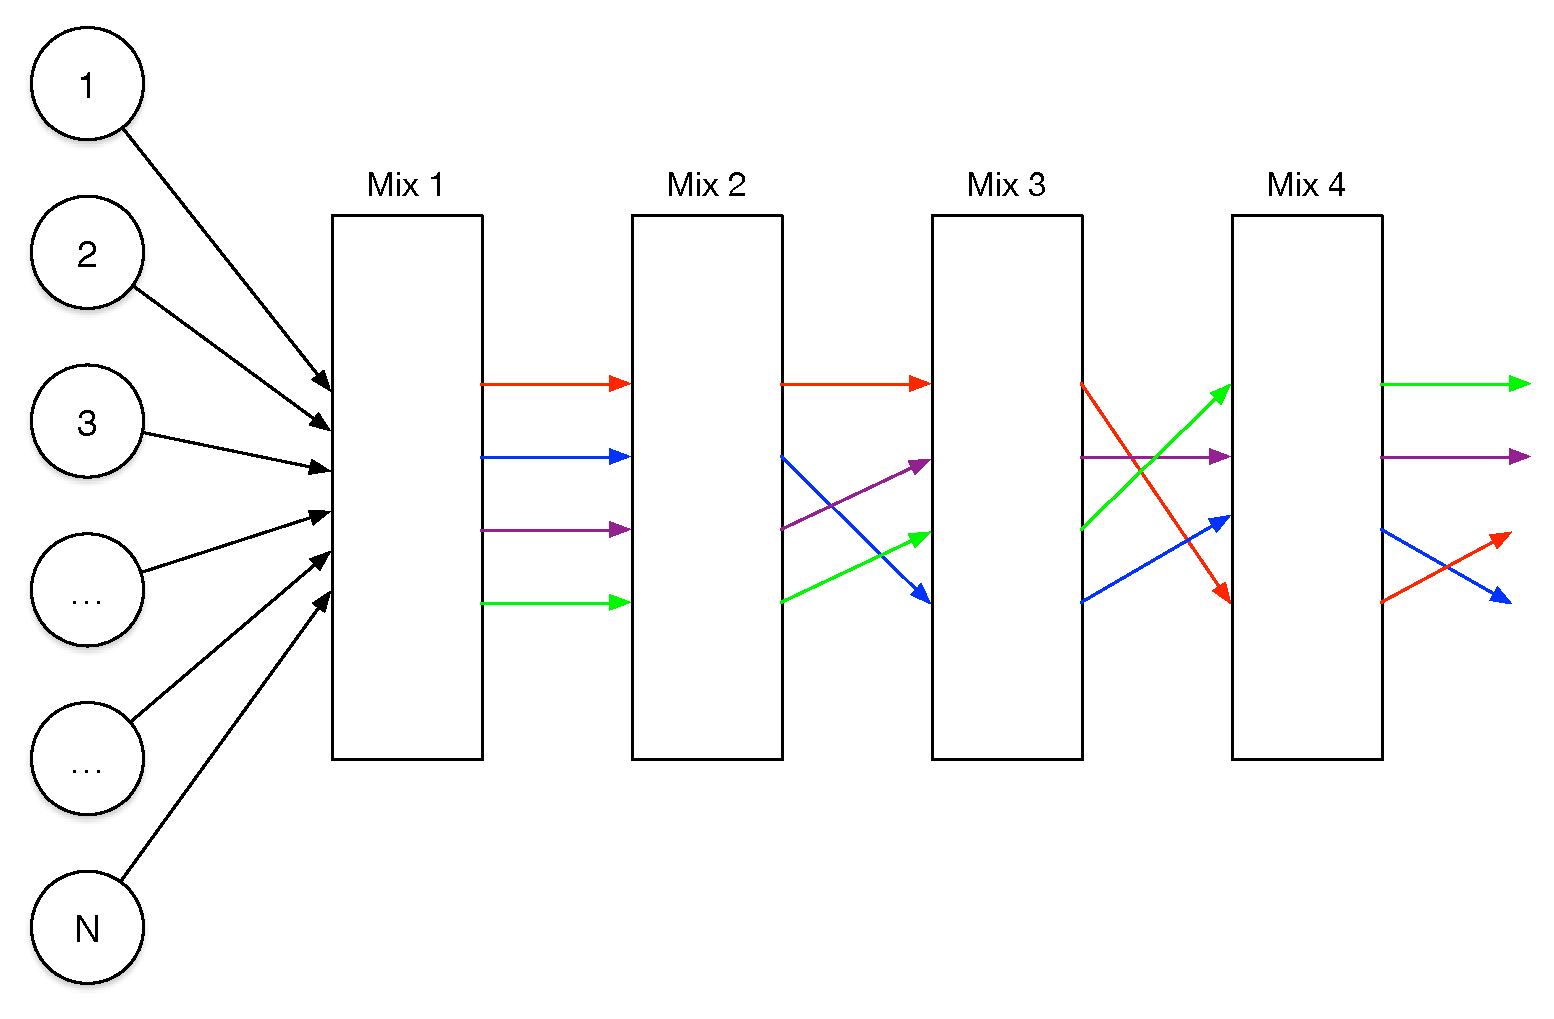
\includegraphics[scale=0.35]{images/mix_design.pdf}
\label{TODO.}
\label{fig:mix-design}
\end{center}
\end{figure}

\begin{figure}
\begin{center}
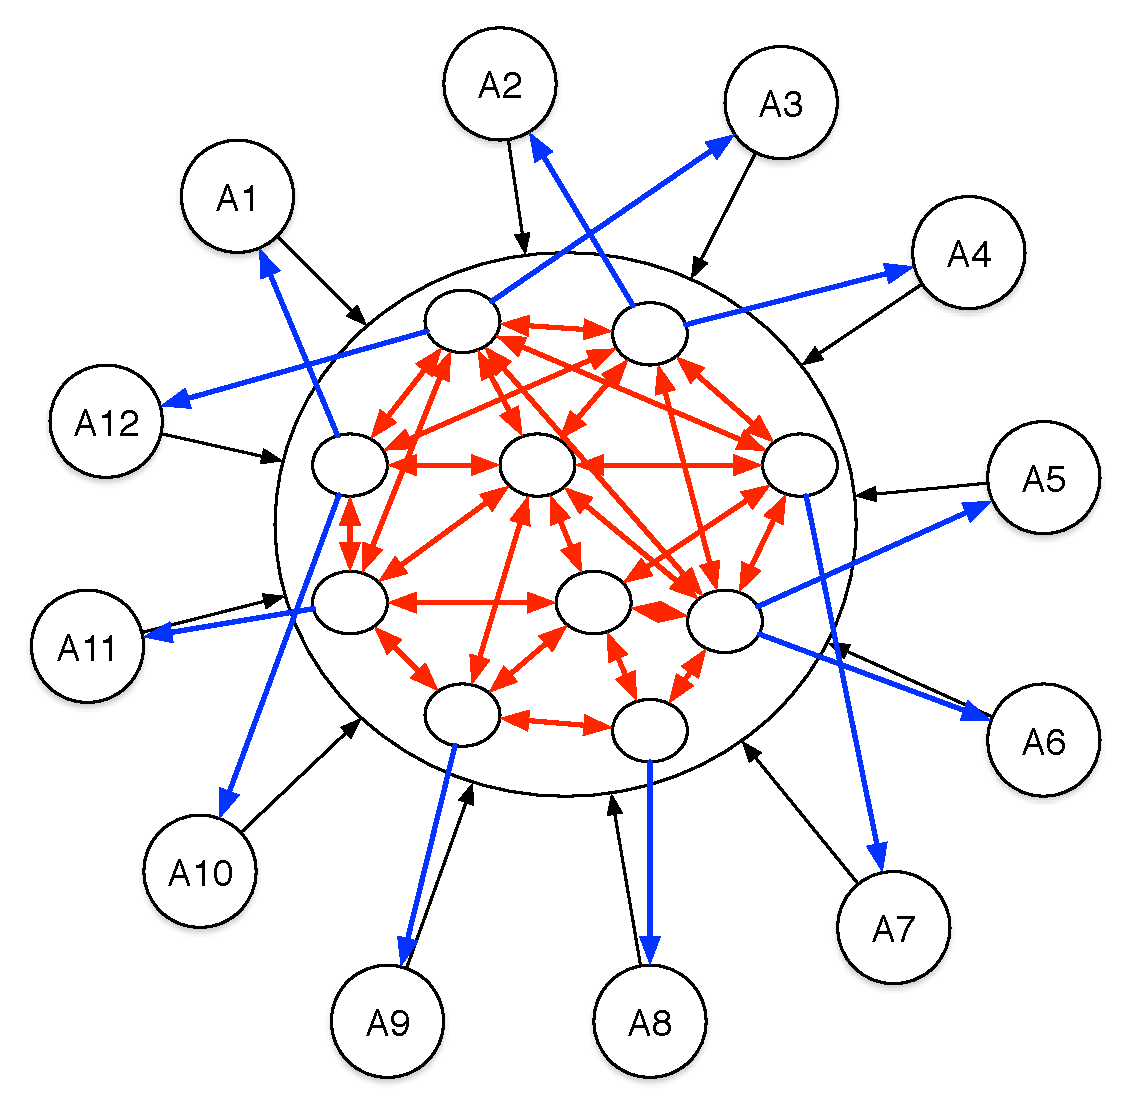
\includegraphics[scale=0.35]{images/mix_bitcoin.pdf}
\label{TODO.}
\label{fig:mix-design}
\end{center}
\end{figure}

Unfortunately, Bitcoin mixing services naturally require a certain level of trust on behalf of the user. In particular, there is nothing in the current Bitcoin system that prevents a malicious mixing service from aggregating a large collection of coins and then abandoning their duty as a mixing service, thereby stealing all of its user's coins. Of course, such financial losses can be minimized if the user only sends funds to the mixing services in small amounts, but it does not eliminate the problem (users would then need to sequentially small small amounts to the mixer, thus drastically increasing the payout time). Therefore, we identify mixing \emph{theft} as a primary threat to users, as well as deanonymization, since the mixing service naturally learns the client's input transaction-signing and output change address.

Given these problems with simple mixing services in the context of Bitcoin, there has been several attempts to modify their usage in order to avoid the aforementioned threats. One work by Barber et al. \cite{BetterToBitter} explored such a modification under the assumption that there does not exist an underlying trust architecture that can be relied upon to prevent the attacks; their conclusion was that the only feasible alternative is to use a \emph{fair exchange protocol} between the users and mixing service to ensure that all input coins are eventually paid back. Unfortunately, their proposed protocol must be integrated with the existing Bitcoin protocol - it is not natively supported. For brefity, we highlight the main features of their approach here. The fair exchange protocol between a sender and mixing service, denoted as parties $A$ and $B$, respectively, requires three types of transactions:
\begin{enumerate}
	\item Commitment transaction to commit a party to a coin exchange.
	\item Refund transaction to refund a party's committed coins at a future date in case the other party aborts the protocol.
	\item Claim transaction to claim the other party's committed money. 
\end{enumerate}
After establishing a set of shared secrets, $A$ and $B$ then begin the fair exchange protocol, which proceeds as follows:
\begin{enumerate}
	\item $B$ generates a committment and refund transaction, with the help of $A$, and broadcasts both transactions. The committment transaction is constructed such that its respective funds can be redeemed using either the corresponding refund transaction (after the protocol ``times out'', or one party fails to complete their duties within a pre-defined ) or a to-be-generated claim transaction. \footnote{The refund transactions are constructed with the output coins being redirected back to their original owner so that the coins are not lost in the event that the protocol does not complete.}
	\item Simultaneously, $A$ generates a committment and refund transaction, also with the help of $B$, and broadcasts both to the network. 
	\item After both parties are committed to the exchange, they must claim their coins. In order to do so fairly, $B$ first claims $A$'s coins using $A$'s refund transaction, and by doing so, enables $A$ to claim $B$'s coins through $B$'s refund transaction. This refund process works as follows: $B$ modifies the output of $A$'s refund script to be redirected to $B$'s recently generated address, and also modifies the input of the script to reveal the ``secret'' values that enable $A$ to modify her refund transcation. Once $B$ publishes his claim transaction, thus taking $A$'s funds, $A$ can then receive the secret values from $B$'s claim transaction to modify $B$'s refund transaction output to point to her own recently generated address. $A$ then broadcasts her claim transaction to claim $B$'s coins, thus completing the exchange.
	\item If a protocol ``timeout'' occurs, then the refund transactions were never properly modified by both parties to steal the other party's coins, and no exchange took place. 
\end{enumerate}
With an existing public key infrastructure and means to securely transfer the secrets used in the transaction generation, this protocol will prevent malicious mixing services from stealing user's coins. However, it requires modifications to the underlying Bitcoin protocol that aren't readily supported. Namely, it requires that transactions support the notion of timelock (i.e., points in time when they can no longer be changed). 

%%% MIXCOIN
Motivated by the desire to achieve the same level of trust without modifying the underlying Bitcoin protocol, Bonneau et el. \cite{mixcoin} recently proposed Mixcoin, a natively-supported protocol for building accountability into mixing services. The principal idea used to achieve mixing accountability is to rely on simple economics, rather than cryptographic solutions, to ensure that mixing services will benefit more from honest participation in mixing rather than from theft. The authors are primarily interested in two main malicious mixing service threats: theft and client deanonymization. Properly aligned financial incentives ensure that theft is not likely to happen (else the mixing service's reputation is permanently destoryed). However, as the authors note, there is not (protocol-level) mechanism that can be used to gaurantee that a mixing service is not linking client input and output addresses; software implementations of mixing services may (purposefully or accidentally) store this information and thus render it susceptible to exposure if compromised. 

%Accordingly, while client deanonymization through mixing services is recognized, it is not solved by Mixcoin. 

The key to achieving accountability through financial incentives is that mixing nodes will provide warranties stating that they claim to complete a mixing operation prior to some agreed-upon deadline. If the mixing node operates dishonestly or steals the client's funds, the client then simply broadcasts the warranty to the network, which is signed by the mixing node using a long-term private key, which can then be verified by all nodes in the network using the corresponding mixing node's public key. The net effect is that no more (intelligent) clients will do business with the mixing node. Since mixing nodes are paid for their efforts through a mixing fee, with an appropriate fee selection it is therefore economically sensible to behave honestly rather than attempt to steal funds. 

The fundamental protocol used to achieve this accountability operates as follows:
\begin{enumerate}
	\item A client $A$ generates a tuple $T = (v, \mathsf{addr}_{\mathsf{in}}, \mathsf{addr}_{\mathsf{out}}, t_1, n)$, where $v$ is the BTC amount to send, $t_1$ is a time by which $A$ will transfer the $v$ funds, and $n$ is a random nonce. This tuple is then sent to the mixing node $M$.
	\item If $M$ accepts the parameters, a fresh escrow address $\mathsf{addr}_{\mathsf{escrow}}$ is generated at which the funds can be acquired by $M$, a deadline $t_2$ by which the funds will be transferred, and a mixing fee rate $p$. These parameters are then signed using the long-term key $K_M$ to generate a warranty, and both are then sent to $A$.
	\item If $A$ accepts $t_2$ and $p$, $A$ transfers the funds to $\mathsf{addr}_{\mathsf{escrow}}$.
	\item After receipt of the funds at $\mathsf{addr}_{\mathsf{escrow}}$, $M$ will return the same amount of funds, minus the agreed-upon transaction fee, to $\mathsf{addr}_{\mathsf{out}}$.
	\item Both parties delete the parameters used in the transaction.
\end{enumerate}

Observe that a client may choose to opt out of the protocol at any point prior to the transfer of the funds by $A$. If $M$ does not act honestly, $A$ simply broadcasts the signed warranty to other nodes so that they may see $A$ was cheated. It is also important to note that, just as in traditional mixing schemes, these mixing nodes may be used sequentially to increase anonymity through multiple mixing rounds. This is done by using the output address of the $i$-th round of mixing as the input address of the $(i+1)$-th round, thereby creating a chain through which the client's funds flow through potentially separate mixes. 

While simple, there are several underlying issues that must be addressed in practice to ensure anonymity:
\begin{itemize}
	\item All Bitcoin chunk sizes should be uniform;
	\item Transaction fees should be randomized (from an appropriate source of randomness, such as a Beacon \cite{nist-beacon} or some PRG computed based on the transaction block chain);
	\item There should never be two outstanding warranties for the same input address issues at the same time;
	\item Clients should not publicize their freshly created input addresses until mixing has initiated, else a malicious party could perform a DoS attack (due to the above requirement) by requesting a warranty for some observed or predicted input address;
\end{itemize}

A brief analysis of the anonymity properties provided by Mixcoin was also presented. Of the most trivial observations are that mixing message replay is impossible due to the single-warranty issuance property stated above, and also that blocking client-to-mix or mix-to-client transactions is not feasible under the standard assumption that the majority of Bitcoin users and miners are not malicious. They also derived a value for the maximum mix delay $\delta_{max}$ (i.e., the time between receiving input funds and transferring output funds) to optimize the client's anonymity set. If a mix receives a input transactions at a stable rate where $Q$ chunks are mixed in a single round (i.e., the total number of funds mixed is equal to $Q \times v$, where $v$ is the uniform mixing input), then the anonymity set of each client is roughly $Q(\delta_{max} - w + 1)$, since fresh input and output keys are used for each of the $Q$ chunks for a particular user, and where $w$ is the minimum difference between $t_2$ and $t_1$ (observe that the final mix delay, uniformly generated, thus falls in the interval $[w, \delta_{max}]$). For $98 \leq Q \leq 4096$, it was found that $\delta_{max} = 7$ since the anonymity set grows by $1 + \frac{\log_2Q(\delta_{max} - w + 1)}{1 + w + \frac{\delta_{max} - w}{2}}$; see Figure \ref{fig:mixcoin-delay-plot}.

\begin{figure}
\begin{center}
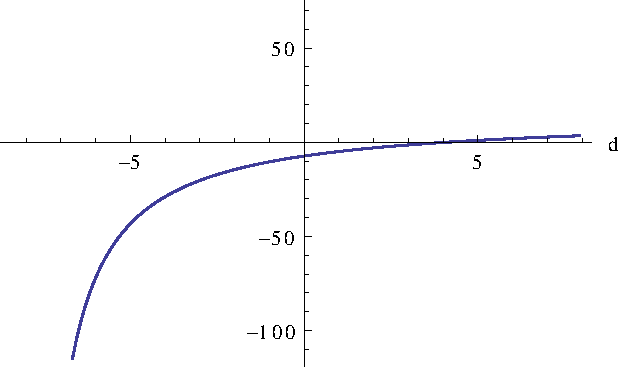
\includegraphics[scale=0.75]{images/mixcoin-delay_plot.pdf}
\label{TODO.}
\label{fig:mix-design}
\end{center}
\end{figure}

%% TODO: mixcoin section 5.4 finish up

\begin{figure}
\begin{center}
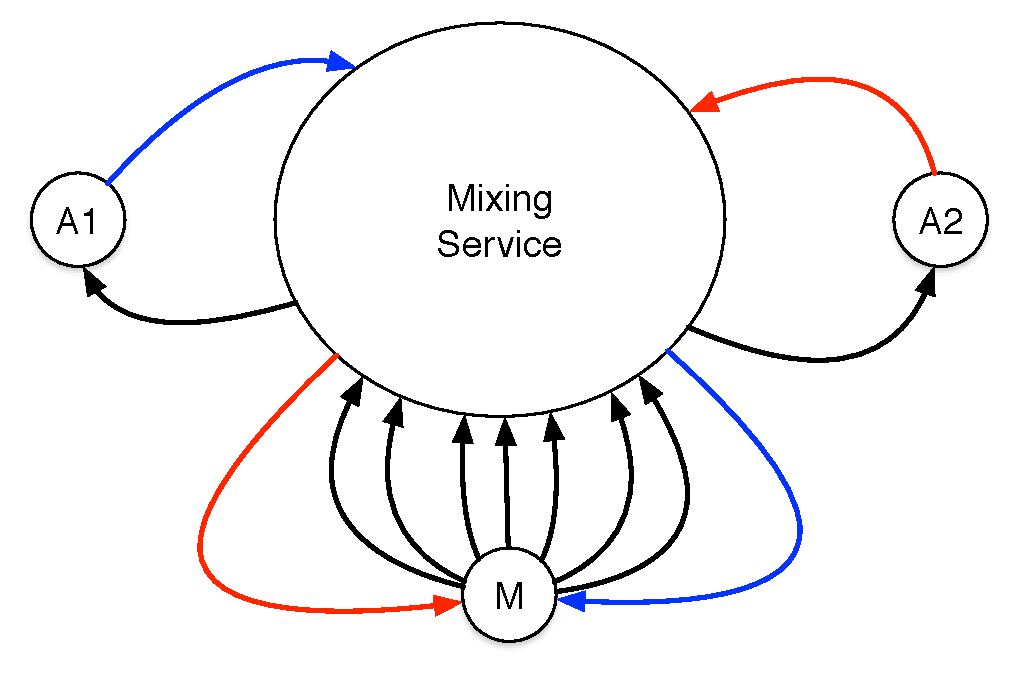
\includegraphics[scale=0.45]{images/mixcoin_deanon.pdf}
\label{TODO.}
\label{fig:mix-design}
\end{center}
\end{figure}

\subsection{Cryptographically-Enhanced Protocols for Anonymity on Top of Bitcoin}

%%% ZEROCOIN
The underlying idea behind the Zerocoin protocol is amazingly simple and intuitive, and it stems from the fact that Bitcoin transactions are publicly linked together and therefore susceptible to passive network analysis techniques (as previously discussed above). Zerocoin breaks the links between transactions using cryptographic techniques that yield the same property of Bitcoin transaction chains (namely, the flow of coins and current value of a transaction). Ultimately, Zerocoins are not identified by public keys as in the case of the backing Bitcoin currency; rather, they are identified by a commitment $C$ to randomly generated secrets (i.e., a serial number $S$ associated with the coin and ``opening value'' $r$) only maintained by the owner of the coins. To do this, Zerocoin leverages accumulators, or primitives that enable a party to sign a collection of objects as opposed to a single object and accumulate the result into a single signature digest (in this case, the collection would be the set of previous transactions), and zero-knowledge proofs. 

The use of these cryptographic techniques as follows. Whenever a user wants to spend Zerocoins they receive associated with some committment $C$, the owner must reveal $S$ publicly and then provide a proof that they are also in possession of $r$ capable of opening some commitment $C_i \in \{C_0,\dots,C_{n-1}\}$, the set of all committments made in the system. The owner uses $r$ to generate a (zero-knowledge) ``signature of knowledge'' $\pi$ that is equivalent to stating that the owner can open some committment (coin) $C_i \in \{C_0,\dots,C_{n-1}\}$, without revealing which coin they actually own (hence, the signature of knowledge is actually a zero-knowledge proof). Technically, to generate this proof, the owner accumulates the results of all coins used to finance the transaction into an RSA-based accumulator, produces an accumulator witness $w$ (the accumulated total of all bitcoins in the transaction minus the value of the Zerocoins to be spent), and finally, generates $\pi$ that enables other entities to \emph{publicly} verify that the value in the accumulator was generated by the entity who derived this proof and was in possession of the Zerocoins coins (committments) necessary to fund this transaction. Zerocoin peers can then verify an accumulated value, representing virtually the same information as a Bitcoin transaction graph, using $\pi$.

From an anonymity perspective, Zerocoin ensures that given two Zerocoins and one ``spend'' coin, one is not able to determine, using publicly available knowledge, which coin was spent (i.e., the adversary's advantage in correctly identifying the spent coin is negligible in the security parameter of the system). With respect to the size of anonymity set, this means that $k = 2$, which is ideal. However, in practice, Zerocoin is inherently limited in that the size of the spender anonymity set can be significaly reduced under certain circumstances. For example, if a user mints and subsequently spends $5$ Zerocoins, it is clear to an adversary participating in the system that all $5$ coins were spent since they can simply verify the transactions; the adversary does not, however, know which coin was spent in which transaction, implying that the anonymity set cardinality is $k = 5$. Now, if the same user not mints and spends another coin, one would hope that the anonymity set would increase to $k = 6$. Clearly, this is not the case, as the attacker can easily deduce that the last minted coin was spent in the last transaction, and thus $k = 1$. Therefore, the anonymity set cardinality for a single coin is clearly bounded below by the number of coins minted between the time of the candidate coin's mint and spend, and upper bounded by the total number of minted coins in the system. Other anonymity issues of Zerocoin relate to the fact that all minted and spent coins are public knowledge, and that all transaction denominations are also publicly available. These can easily be addressed in practice, however.

%TODO: image of accumulation and verification

The mathematical details of accumulation and witness verification are not discussed for brevity. However, we note that security of both schemes relies on the hardness of the Strong RSA and Discrete Logarithm assumptions. As such, the operations required for accumulation and verification come at the cost of additional computational overhead. Furthermore, Zerocoin requires a preliminary, potentially offline, setup phase in which the parameters for the accumulator and zero-knowledge scheme. Aware of these pitfalls, the authors propose a variety of optimizations for improving Zerocoin performance. Namely, they introduce the notion of accumulator checkpoints, which are essentially timestamps that cryptographically capture the value of an accumulator after each transaction in a recently mined block, thus removing the need for a verifier to re-compute the entire accumulator value from scratch upon every invocation. 

Secondly, the authors discuss methods in which the zero-knowledge proof scheme can be improved. Their preliminary experiments revealed that the size of proofs often exceeded the MTU of Bitcoin transactions, which prohibits its immediate use since Zerocoin relies on Bitcoin for the initial source of Zerocoin funds (i.e., Bitcoins are used to mint Zerocoins) and transaction block graphs to timestamp the state of the system. Rather than modify this MUT limitation so that proofs can be stored alongside accumulator checkpoints in the transaction block chain, the authors propose to store and access proofs using a distributed hash table or non block-chained storage mechanism in Bitcoin. With respect to the computational cost of proofs, the authors propose a distribtued verification strategy so as to not make every node verify the proof of every new transaction block. Doing so would be a large computational burden on verifiers, which should be quick, as opposed to miners, whose efforts are justified via transaction fees. Internally, the chosen zero-knowledge signature of knowledge scheme consists of $n$ repetitions of the same proof to reduce the probability of forgery to $\mathcal{O}(2^{-n})$, and so by requiring that each node \emph{randomly} selecting a subset of these $n$ proofs to compute and it is possible to achieve the same proof security guarantee with a significantly reduced amount of duplicated effort.

%% TODO: issues of incremental deployment

%%% Pinocchio Coin
Pinocchio Coin \cite{pinocchio} is an attempt at optimizing the Zerocoin protocol. Whereas Zerocoin uses an accumulator based on the Strong RSA assumption and proofs founded on double discrete logarithms, Pinocchio Coin uses elliptic curves and bilinear pairings to achieve virtually the same behavior with significantly less overhead. As such, Pinocchio Coin follows the same process as Zerocoin for {\sf setup}, {\sf mint}, {\sf spend}, and {\sf verify} coins: The setup phase involves creating a suitable pairing-friendly elliptic curve in the security parameter and then configuring the parameters for the Pinocchio proof system. As previously stated, minting, spending, and verification are analogous to the Zerocoin protocol with the exception that proofs are generated without the need to accumulate past commitments (though the proof generation still requires all commitments $C_0,\dots,C_{n-1}$ as input to ensure correctness). The output of the spend procedure 

The Pinocchio proof of work was originally designed as a generic proof of work to be used in applications such as cloud computing. The system takes a set of operations and converts them into proof of work that can be seen as a zero knowledge proof. The primary advantage of using Pinocchio Coin over Zerocoin is that the size of each proof is significantly smaller; Pinocchio proofs are less than 400 bytes as opposed to Zerocoin's 50kB proofs, which are well within the Bitcoin transaction size limits. One potential disadvantage of using Pinocchio Coin are that there is no security analysis as of yet \cite{pinocchio}. Futhermore, although Pinocchio serves as an efficient general proof compiler, it is unknown if specialized systems, such as ZKPDL, would exhibit better performance in the Zerocoin framework.

%%% COINJOIN
CoinJoin \cite{coinjoin} is a method to have multi-user inputs in a Bitcoin transaction. Users agree on a common output size and then combine all their transactions of that size into one big transaction. The aim of this method is to obfuscate which user is the input to an output and prevent the association of multiple addresses in a transaction to one user.

It is not be clear which user is associated to a certain output if multiple transactions with the same sized output are combined together. Any user could have paid for any output. For instance, if Alice has a 1 Bitcoin transaction to Carol and Bob has a 1 Bitcoin transaction to Dave, they can combine their transactions together to create one transaction with two outputs for 1 Bitcoin each. Now it is unclear if Alice paid Carol or Dave. With more simultaneous users, the ability to accurately track transactions would decrease.

CoinJoin allows for multiple inputs per user and combines them all into one transaction. With enough users, the transaction would hide which of the many accounts belong to which user. Although some analysis can be done on the inputs and outputs, it would not have nearly the same accuracy as the current heuristic of one user per transaction.

The simplest implementation of CoinJoin can be done with a ``meet-up'' server to coordinate transactions. A decentralized version can be used, but the issues with coordinating transactions cause complexity.

The most notable feature of CoinJoin, aside from privacy, is that it works today \emph{without} any modification to the Bitocoin protocol, which is untrue for solutions akin to Zerocoin. The transactions from CoinJoin are identical to normal Bitcoin transactions. A potential development involves moving away from a centralized server that knows all the mappings to one that doesn't and eventually a de-centralized system. It is also unknown how many sessions does the protection of privacy extends. Finally, CoinJoin similar to other financial systems, CoinJoin does not hide the user's IP address; an anonymity layer such as Tor is needed to obfuscate this information from a sender's peers.

%%%%%%%%%%%%%%%%%%%%%%%%%%%%%%%%%%%%%%%%%%%%%%%%%%%%%%%%%%%%

%Centralized mixes similar to Chaums anonymous email (BitFog, BitLaundry, Blockchain.info) and decentralized mixes (Zerocoin).

% The anonymity problem in Bitcoin was later addressed by ZeroCoin [13] which allows the implementation of a Zero- Knowledge based decentralized coin mixing service. Earlier Hanke et al. [10] presented a Pay-to-Contract Protocol that is built on top of Bitcoin and secures transactions between
% merchants and their clients. CommitCoin [6] is another system that builds on the blockchain to carbon date commitments.

%[5]Dorit Ron and Adi Shamir. Quantitative Analysis of the Full Bitcoin Transaction Graph. IACR Cryptology ePrint Archive 584 (2012).

%[6] Sarah Meiklejohn, Marjori Pomarole, Grant Jordan, Kirill Levchenko, Damon McCoy, Geoffrey M. Voelker, and Stefan Savage. 2013. A fistful of bitcoins: characterizing payments among men with no names. In Proceedings of the 2013 conference on Internet measurement conference(IMC '13). ACM, New York, NY, USA, 127-140

%[7] Fergal Reid and Martin Harrigan. 2013. An Analysis of Anonymity in the Bitcoin System. Security and Privacy in Social Networks. Springer, New York, NY, USA, 197-223

%[8] Dan Kaminsky. 2011. Black Ops of TCP/IP 2011. Black Hat USA 2011. http://www.slideshare.net/dakami/black-ops-of-tcpip-2011-black-hat-usa-2011

%[9] Malte Moser. 2013. Anonymity of Bitcoin Transactions: An Analysis of Mixing Services. Munster Bitcoin Conference (MBC). July 17-18, Munster, Germany




%attacks on address indistinguishabiilty include multi-address transactions and shadow/change accounts
% Researchers attempt to break the anonymity of Bitcoins in an attempt to study stolen Bitcoins [6][8]. In a similar manner to the attack on privacy, a user graph is created. 
%There is research between big data (the user and transaction graphs) and re-identifying people. Netflix and social networks (Broken Promise of Privacy: Responding to the Surprising Failure of Anonymization by Paul Ohm and De-anonymizing Social Networks by Arvind Narayanan and Vitaly Shmatikov).  Is this outside the scope of our paper? It's alluded that user transaction graphs can be used to identify real world identities, but no one has done it yet.